\section{Results}
\label{sec:results}


The proposed trajectory generation algorithm was integrated into our own crowd patches platform in C++.
Each of the experiments described in the following paragraphs were for patches of size $A = 16m * 16m$ and period $\pi = 10sec$.
% We evaluate the proposed method both qualitative and quantitatively.

\textbf{Performance}
% As expected, increasing the number of initial control points increases the time required for the algorithm to converge to collision free trajectories (Figure~\ref{fig:res:performance}) due to increased crowd density.
All the performance measurements presented in this section were run on a single thread of an Intel Xeon quad core $2.8$ GHz processor having $8$GB of RAM (Figure~\ref{fig:res:performance}.
% For the results presented here , patches had an area of $A = 16m * 16m$ and period $\pi = 10sec$.
Each experiment consisted of placing equal numbers of entry/exit points in random positions around the border of the patches.
For each possible number of entry/exit points (ranging from $1-50$) the experiment was run multiple times ($20$) resulting in $1000$ different patches.
For each one of the experiments, time and number of iterations required for convergence were measured.
The results indicate a direct correlation of the number of iterations to the time required for convergence.
More importantly, increasing the number of control points decreases performance exponentially due to increased density.

Additionally, some of the experiments having more than a total of $60$ control points ($0.6\%$ of the experiments) had very slow convergence and were forced to stop at $2000$ iterations resulting in some collisions in the patch.
Examining the patches that failed to converge we observed that these was mainly due to the placement of the initial control points; if control points are clustered on a subset of the patch's sides matching between them is more difficult and non-optimal.
To account for this (assuming that the whole crowd patch generation is completely automatic) a better control point generation algorithm must be implemented.



% Performance was measured on a computer with an Intel Xeon quad core 2.8 GHz processor and 8GB of RAM. We found trajectories for patches with randomly generated entry and exit points. The patches all had base square of size 16 by 16. The period was 10 seconds. There were 20 samples for each number of agents between 1 and 50 for a total of 1000 samples. 994 of these were collision free. The other 6 were stopped after they reached 2000 iterations. We recorded the number of iterations required for collision free trajectories as well as the computation time in seconds.

%%----------------------------------------------------------------
%% Figure: Performance
%%----------------------------------------------------------------
\begin{figure*}[t]
 \centering
%
\begin{subfigure}[b]{0.48\linewidth}
 \centering
	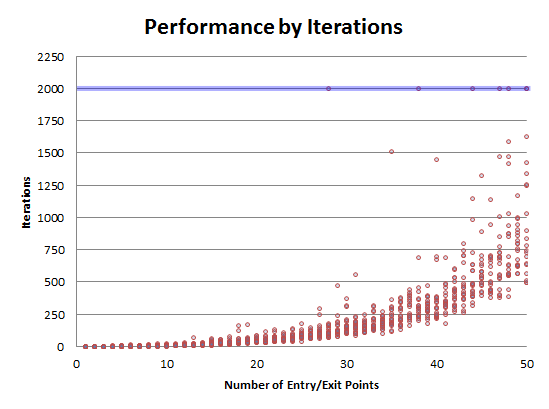
\includegraphics[width=\linewidth]{images/res-iter-graph.png}
	\caption{}
 \end{subfigure}
%
\begin{subfigure}[b]{0.48\linewidth}
 \centering
	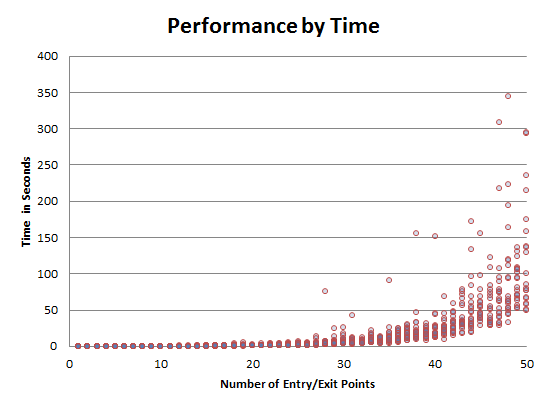
\includegraphics[width=\linewidth]{images/res-time-graph.png}
	\caption{}
 \end{subfigure}
% 
\caption{
		\textbf{Performance}
		A dot on each graph represents a simulated patch.
		(a) The number of iterations for the proposed algorithm to converge is exponential to the number of initial control points -- some of the experiments failed to converge.
		(b) Time is directly correlated to the number of iterations.
% 		The patch had a specified number of entrance and exit points whose locations were randomly generated.
% 		Our algorithm was run until either the patch was collision free, or it reached 2000 iterations. 
% 		(a) The number of iterations was recorded in relation to number of Entry/Exit Points. The blue line at 2000 iterations shows where the simulation was stopped (6 out of 1000 patches were stopped here, and thus were not collision free).
% 		(b) The time to converge was measured in seconds.
}
% \\\\ //each experiment needed to converge whereas the blue horizontal line indicates the maximum number of allowed iterations ($6$  out of $1000$ inputs \panayiotis{What do we mean by inputs? experiments or the total number of trajectories. Does this graph show how much time it took for a whole patch or for the trajectories with collisions?} didn't converge after $2000$ iterations) . \textbf{(b)} The time to converge was measured in seconds.  \devin{should I remove the titles on the images of the graphs, and instead put their title in the caption?} \panayiotis{No, you should leave them.. If you can edit the images, please remove the borders. I think it will look nicer. Also, this graphs confuse me a little bit. We should discuss them with Guillermo - I want to get a feeling of what exactly are we showing here}
\label{fig:res:performance}
\end{figure*}
%%----------------------------------------------------------------
%% Figure: Performance
%%----------------------------------------------------------------



\textbf{Example visualization}
The proposed method manages to create trajectories that are both free of collisions and with smooth motion; i.e., agents following these trajectories have speeds near regular humans comfort speeds and are also visually pleasing.
Figure~\ref{fig:res:steps} shows the trajectories generated by the proposed method for a patch consisting of $10$ input and $10$ output points and the intermediate steps; first input and output points are matched and connected with linear trajectories using Algorithm~{\ref{alg:stable-matching}}, then any collisions are handled using Algorithm~\ref{algo:control-points} and finally the generated trajectories are smoothed out.

%%----------------------------------------------------------------
%% Figure: Steps
%%----------------------------------------------------------------
\begin{figure*}[t]
	 \centering
	 \begin{subfigure}[b]{0.24\linewidth}
	 	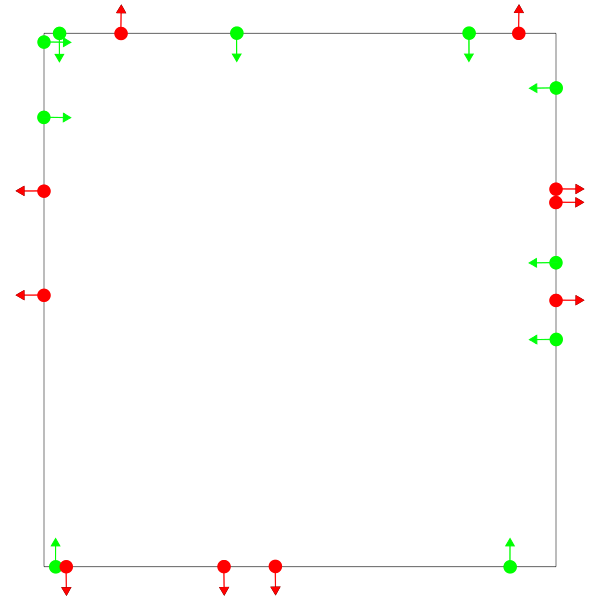
\includegraphics[width=\linewidth]{images/steps-input.png}
	 	\caption{Input}
	 \end{subfigure}
	 % 
	 \begin{subfigure}[b]{0.24\linewidth}
	 	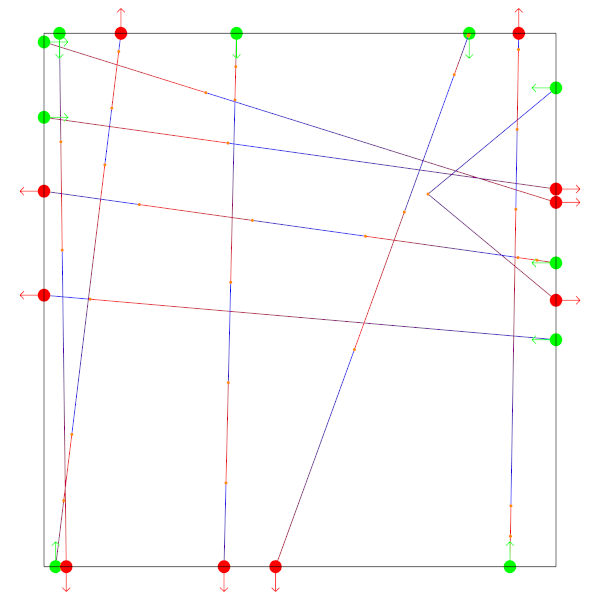
\includegraphics[width=\linewidth]{images/steps-connected.png}
	 	\caption{Connected}
	 \end{subfigure}
	 %
	 \begin{subfigure}[b]{0.24\linewidth}
	 	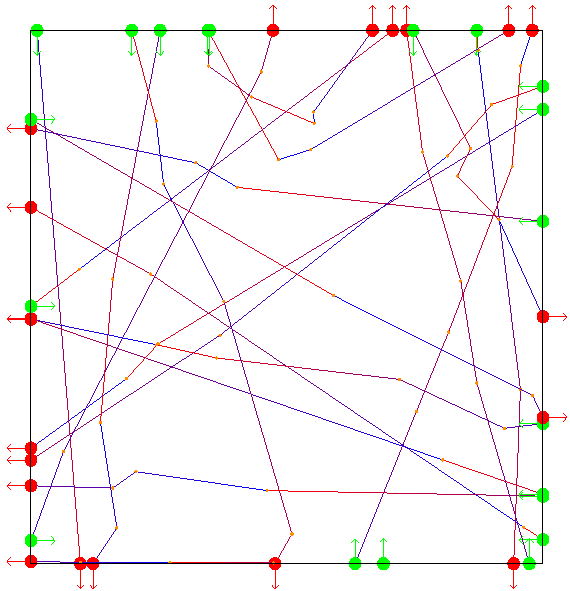
\includegraphics[width=\linewidth]{images/steps-collisionFree.png}
	 	\caption{Collision Free}
	 \end{subfigure}
	 %
	 \begin{subfigure}[b]{0.24\linewidth}
	 	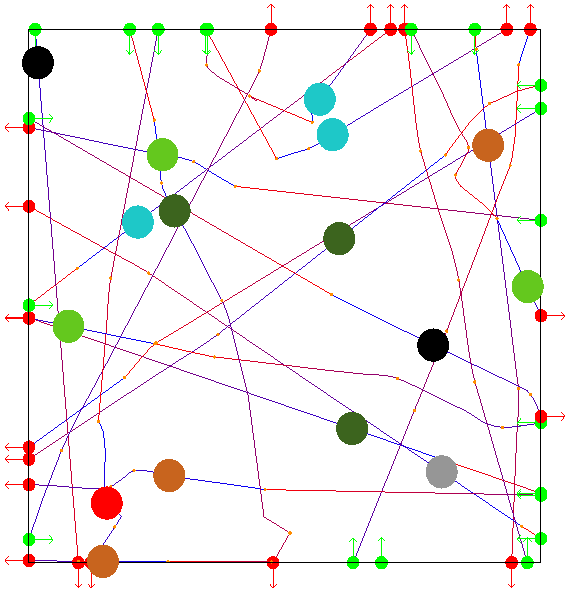
\includegraphics[width=\linewidth]{images/steps-smoothed.png}
	 	\caption{Smoothed Out}
	 \end{subfigure}
	 \caption{\textbf{Method example}
	 			The proposed method starts from
	 			(a) a set of control points in the boundaries of an empty patch,
	 			(b) interconnects them in an optimal way,
	 			(c) resolves any temporal collisions and finally
	 			(d) smooths the trajectories.
	 }
 \label{fig:res:steps}
\end{figure*}
%%----------------------------------------------------------------
%% Figure: Steps
%%----------------------------------------------------------------

\textbf{Adaptability to control point placement}
This method is able to adjust to the placement of the control points (Figure~\ref{fig:res:adapt-cp-placement}) aiming at the same time for good space coverage over the period of the patch.


\begin{figure*}[t]
 \centering
 \begin{subfigure}[b]{0.24\linewidth}
 	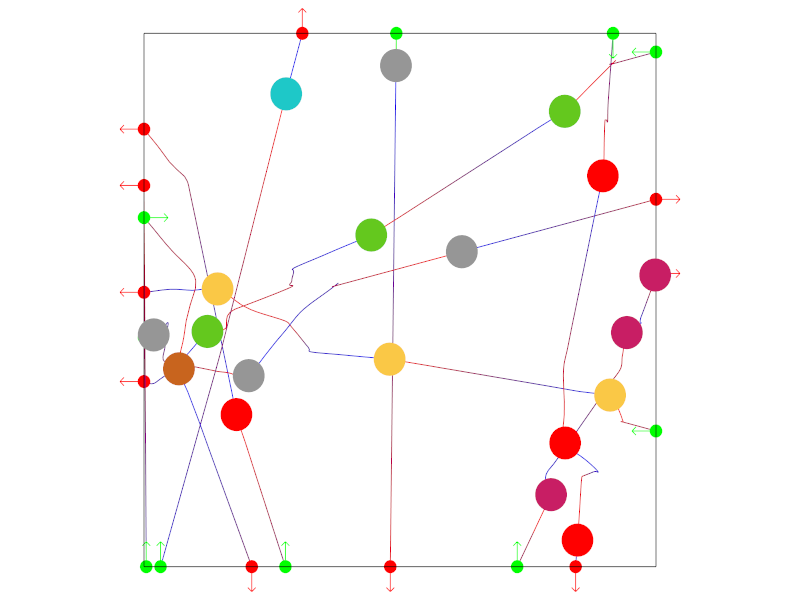
\includegraphics[width=\linewidth]{images/res-10-withAgents_1.png}
 	\caption{}
 \end{subfigure}
 % 
 \begin{subfigure}[b]{0.24\linewidth}
 	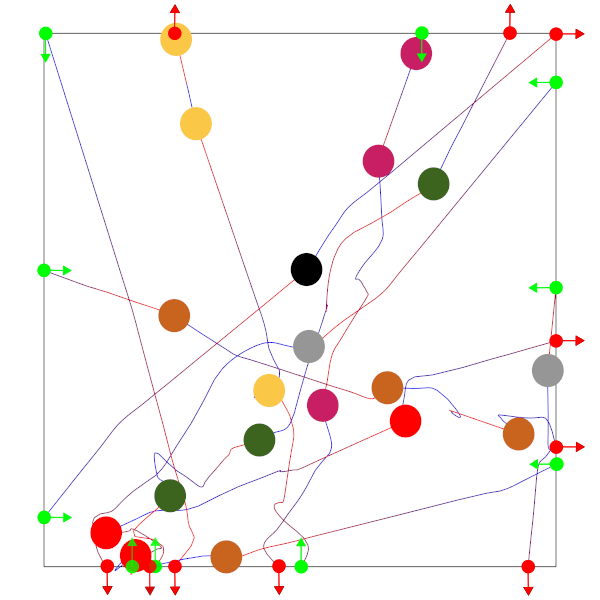
\includegraphics[width=\linewidth]{images/res-10-withAgents_2.png}
 	\caption{}
 \end{subfigure}
 %
 \begin{subfigure}[b]{0.24\linewidth}
 	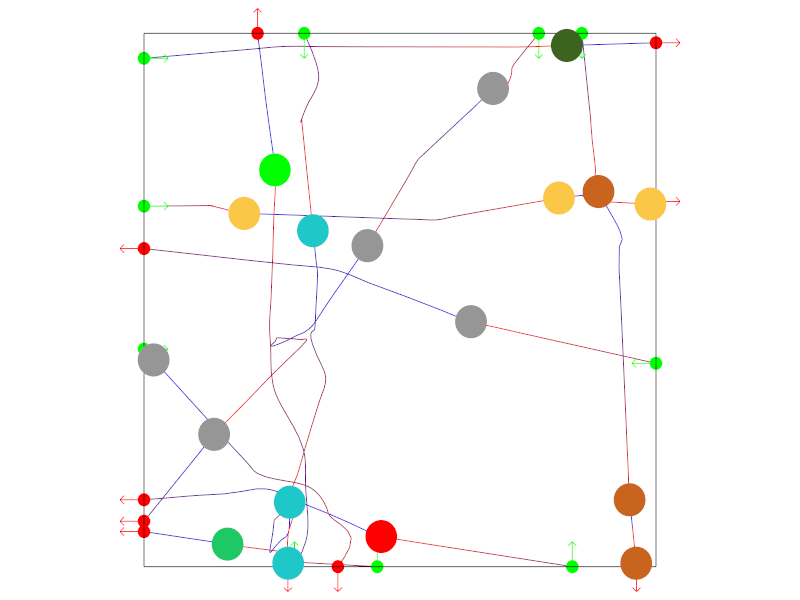
\includegraphics[width=\linewidth]{images/res-10-withAgents_3.png}
 	\caption{}
 \end{subfigure}
 %
 \begin{subfigure}[b]{0.24\linewidth}
 	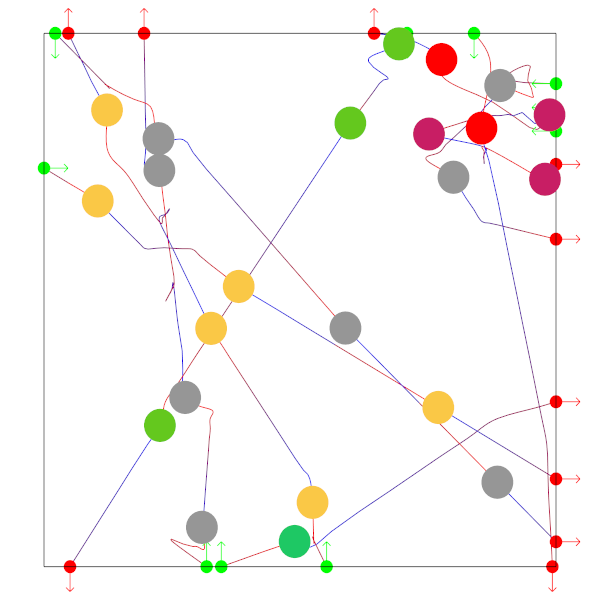
\includegraphics[width=\linewidth]{images/res-10-withAgents_4.png}
 	\caption{}
 \end{subfigure}
 \caption{
 	\textbf{Variance}
 	We demonstrate different results for the same number of initial spatio-temporal control points but different placement.
 	All the examples here consist of $10$ entry and $10$ exit control points.
%  	Several examples showing the final trajectories for 10 Entry/Exit Points
 }
 \label{fig:res:adapt-cp-placement}
\end{figure*}



\textbf{Adaptability to density}
The proposed method can adapt to different numbers of initial control points; i.e., it manages to generate smooth collision free trajectories for increasing larger numbers of trajectories (Figure~\ref{fig:res:inputs}).
Increasing the number of control points increases density and the time required for calculating these trajectories but recall that crowd patches are \emph{precomputed} and therefore during simulation time huge numbers of moving agents can be simulated at limited cost.
Again, trajectories aim to cover the patch's space.



%%----------------------------------------------------------------
%% Figure: Adaptability
%%----------------------------------------------------------------
\begin{figure*}[t]
	\centering
	%
	\begin{subfigure}[b]{0.24\linewidth}
		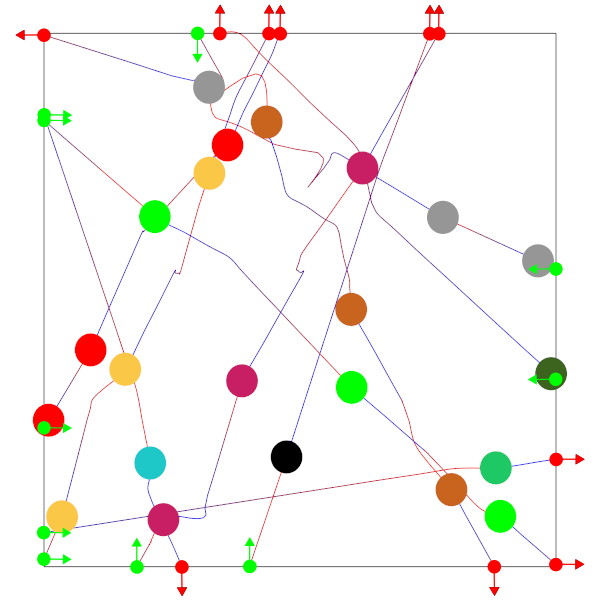
\includegraphics[width=\linewidth]{images/res-10-entry-exit.png}
		\caption{10 Entry/Exit Points}
	 \end{subfigure}
	%
	 \begin{subfigure}[b]{0.24\linewidth}
		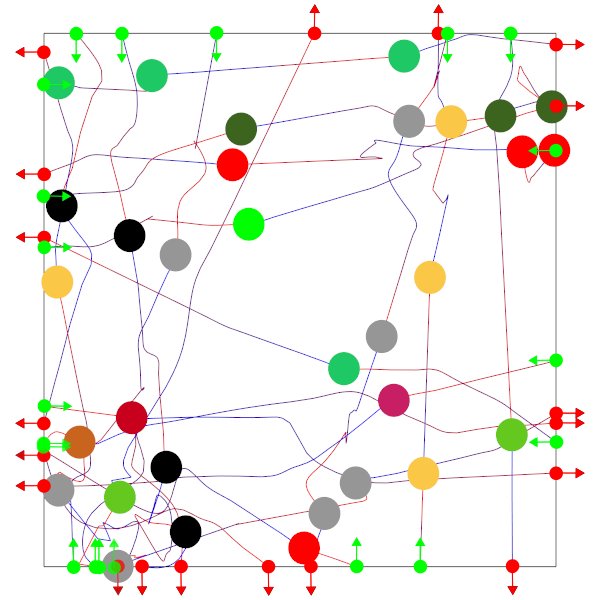
\includegraphics[width=\linewidth]{images/res-20-entry-exit.png}
		\caption{20 Entry/Exit Points}
	 \end{subfigure}
	%
	 \begin{subfigure}[b]{0.24\linewidth}
		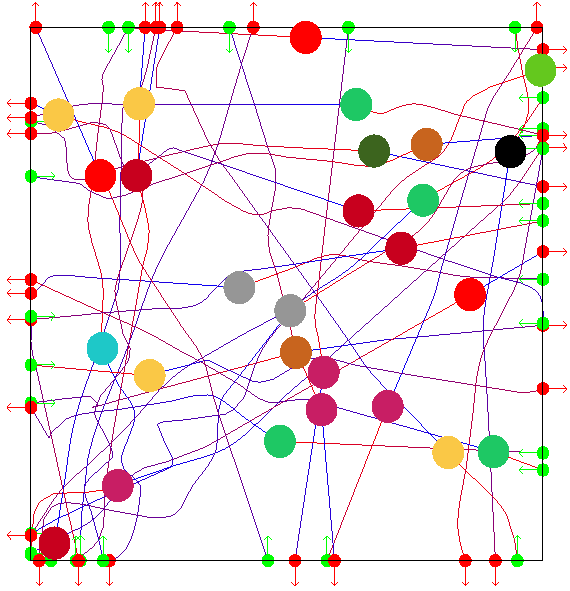
\includegraphics[width=\linewidth]{images/res-30-entry-exit.png}
		\caption{30 Entry/Exit Points}
	 \end{subfigure}
	%
	 \begin{subfigure}[b]{0.24\linewidth}
		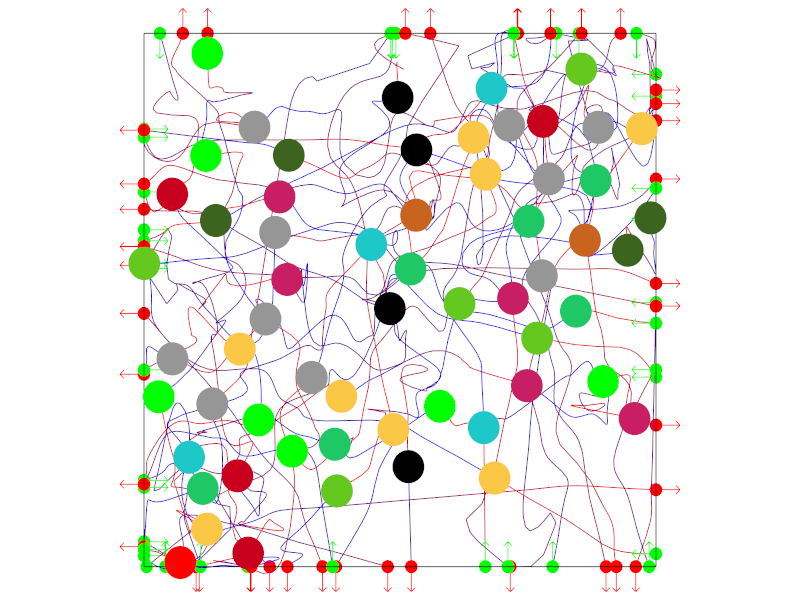
\includegraphics[width=\linewidth]{images/res-40-entry-exit.png}
		\caption{40 Entry/Exit Points}
	 \end{subfigure}
	%
	\caption{\textbf{Density Adaptability}
			The proposed method can generate collision free trajectories for many situations; from sparse to very dense.
			}
	\label{fig:res:inputs}
\end{figure*}
%%----------------------------------------------------------------
%% Figure: Adaptability to density
%%----------------------------------------------------------------


\textbf{Collision Anticipation}
In the original work~\cite{Yersin:2009} Helbing's social forces \cite{Helbing:2005} approach was used to handle collisions.
One problem with that approach is the lack of anticipation by agents; agents handle collisions late resulting in unnatural looking trajectories even for simple scenarios such as the one in Figure~\ref{fig:res:helbing} whereas the proposed approach emulates better anticipatory behaviour.

%%----------------------------------------------------------------
%% Figure: Collision Anticipation
%%----------------------------------------------------------------
\begin{figure}[t]
	\centering
	%
	\begin{subfigure}[b]{0.49\linewidth}
	 \centering
		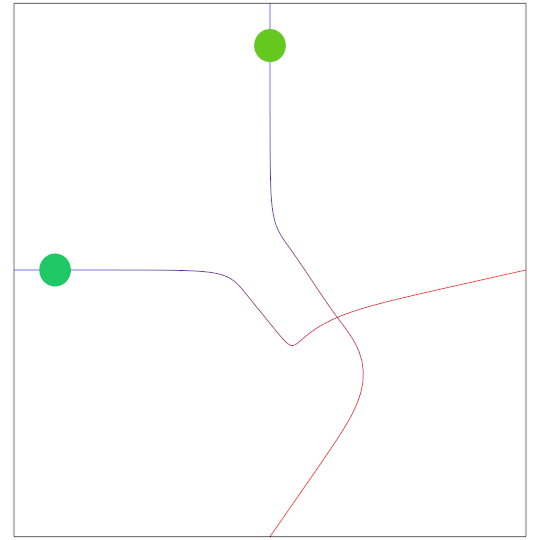
\includegraphics[width=\linewidth]{images/res-helbing-crossing.png}
		\caption{Helbing}
	 \end{subfigure}
	%
	\begin{subfigure}[b]{0.49\linewidth}
	 \centering
		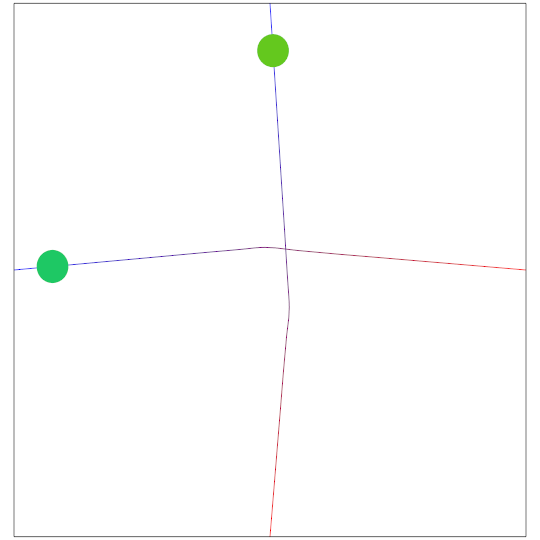
\includegraphics[width=\linewidth]{images/res-iter-crossing.png}
		\caption{Iterative}
	 \end{subfigure}
	% 
	\caption{
		\textbf{Collision Anticipation}
		(a) Using the approach described in \protect \cite{Yersin:2009} trajectories lack anticipation as they suddenly curve when collisions are near whereas
  		(b) the proposed method generates trajectories with higher anticipation resulting in gradually changing direction.
% 		The proposed method manages to generate trajectories with better anticipatory behaviour to \cite{Yersin:2009}
% 		A comparison between both methods, shows the improvement in terms of anticipating a collision. (a) shows little anticipation, it modifies its trajectory until it is about to collide, whereas (b) starts modifying its trajectory gradually from the beginning.
		}
	\label{fig:res:helbing}
%%----------------------------------------------------------------
%% Figure: Collision Anticipation
%%----------------------------------------------------------------
\end{figure}



%In Figure~\ref{fig:res:steps} we have a diagram showing the patch in various steps of our algorithm.
% Next we show the final curved trajectories with various sized input.
% Lastly we show some performance tests.We found that our algorithm created trajectories that were free of collisions and produced smooth motion. In Figure~\ref{fig:res:steps} we have a diagram showing the patch in various steps of our algorithm. Next we show the final curved trajectories with various sized input. Lastly we show some performance tests.











